%\documentclass[compress,dvips,xcolor=table]{beamer}
\usepackage{etex}
%\documentclass{article}
%\usepackage{beamerarticle}
%\usepackage[turkish]{babel}
\usepackage{tikz}
\usetikzlibrary{shapes,arrows,positioning,calc,shadows,matrix,fit}
\usepackage{pgf-umlcd}
\tikzstyle{umlcolor}=[color=\umldrawcolor,fill=\umlfillcolor,text=\umltextcolor,drop shadow]
\usepackage[utf8]{inputenc}
\usepackage{listings}
\usepackage{multicol}
%\includeonlyframes{current}

\def\circtxt#1{$\mathalpha \bigcirc \mkern-13mu \mathtt #1$}

\mode<article>
{
  \usepackage{fullpage}
  \usepackage{pgf}
  \usepackage{hyperref}
}

\mode<presentation>
{
  \usetheme{metuceng}

%  \setbeamercovered{transparent}
}


\title{Programming Language Concepts}
\subtitle{Object Oriented Prog: Polymorphism}
\author{Onur Tolga Şehitoğlu}
\institute[ODTÜ]{Bilgisayar Mühendisliği}
\subject{Object Oriented Prog: Polymorphism}
\date{}
	\titlegraphic{\insertmetutitle\insertlicense}


\begin{document}
\lstset{language=C,
        basicstyle=\scriptsize\ttfamily,
        keywordstyle=\color{blue!50!black}\bfseries,
        identifierstyle=\color{blue!60!green}\sffamily,
        stringstyle=\color{red!70!green}\ttfamily,
	commentstyle=\color{blue!30!white}\itshape,
        showstringspaces=true}
\setbeamercolor{hexample}{bg=green!5!white,fg=black}%
\setbeamercolor{cexample}{bg=blue!5!white,fg=black}%
\setbeamercolor{pexample}{bg=orange!5!white,fg=black}%
\setbeamercolor{oexample}{bg=violet!5!white,fg=black}%

 \frame[plain]{\maketitle}
 \begin{frame}
 \frametitle{Outline}
 \begin{multicols}{2}
 \tableofcontents
 \end{multicols}
 \end{frame}

\defverbatim[colored]\codePolyStatic{
\begin{lstlisting}[language={C++},escapechar=\#]
class A { int x;
public: void get() { cout << 'A::get()';}
};
class B : public A { int y;
public: void get() { cout << 'B::get()';}
}
...
A a, *p;
B b;
p=&a; p->get();	
p=&b; p->get();	
\end{lstlisting}}

\section{Polymorphism}
\begin{frame}
\frametitle{Polymorphism}
\begin{itemize}
	\item Inheritance $\rightarrow$ inclusion polymorphism
	\item Binding is still \structure{static}, at compile time
	\item Pointers of derived classes are converted to superclass types
\begin{beamercolorbox}{cexample}
\codePolyStatic
\end{beamercolorbox}
\end{itemize}
\end{frame}

\defverbatim[colored]\codePolyLate{
\begin{lstlisting}[language={C++},escapechar=\#]
class A { int x;
public: #\alert{virtual}# void get() { cout << 'A::get()';}
};
class B : public A { int y;
public: void get() { cout << 'B::get()';}
}
...
A a, *p;
B b;
p=&a; p->get();	
p=&b; p->get();	
\end{lstlisting}}
\begin{frame}
\frametitle{Late Binding}
\begin{itemize}
	\item Delaying binding possible
\begin{beamercolorbox}{cexample}
\codePolyLate
\end{beamercolorbox}
	\item binding of \structure{virtual} member functions done at run time.
\end{itemize}
\end{frame}

\subsection{Abstract Classes}
\begin{frame}
\frametitle{Abstract Classes}
\begin{itemize}
\item	\lstinline!void f() = 0 ;! makes the function an \structure{abstract member}
\item A class with at least one abstract member is an \structure{abstract class}.
\item Abstract classes cannot be instantiated
\item A derived class remains abstract unless all abstract members are implemented somewhere in derivation chain.
\item Java \structure{interfaces}: abstract classes with only abstract member functions and constants.
\end{itemize}
\end{frame}


\defverbatim[colored]\codeShape{
\begin{lstlisting}[language={C++},escapechar=\#]
class Shape { int x,y;
public: virtual void draw() = 0;
	void move(int a, b) {
	 	setbgcolor(); #\alert{draw()}#;
		x=a; y=b; setfgcolor(); #\alert{draw()}#;
	}
};
class Circle : public Shape { int r;
public: void draw() { /* draw circle here */ }
}
class Rectangle : public Shape { int w,h;
public: void draw() { /* draw rectangle here */ }
}
...
Circle a(...); Rectangle b(...);
a.move(2,4); b.move(3,4);
\end{lstlisting}}
\begin{frame}
\begin{itemize}
	\item binding of \lstinline!move()! is static but the
	\lstinline!draw()!'s inside are still late.
\begin{beamercolorbox}{cexample}
\codeShape
\end{beamercolorbox}
\end{itemize}
\end{frame}

\subsection{Interfaces}
\begin{frame}
\frametitle{Interfaces}
\begin{columns}
\begin{column}{70mm}
\begin{itemize}
\item Java does not have multiple inheritance but a class can 
\structure{implement} multiple interfaces
\item Functions working on interfaces provide polymorphism
for the classes implementing them
\item \lstinline!Person! and \lstinline!Complex! implements the
	interface \lstinline!Sortable! so that \lstinline!sort(...)!
	can work uniformly on both
\end{itemize}
\end{column}
\begin{column}{55mm}
\scriptsize
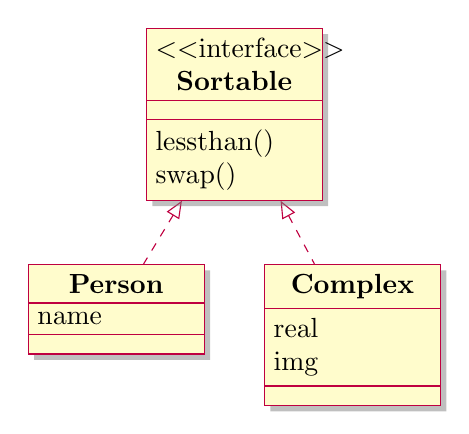
\begin{tikzpicture}
\begin{interface}[text width=2cm]{Sortable}{1.5,3}
\operation{lessthan()}
\operation{swap()}
\end{interface}
\begin{class}[text width=2cm]{Person}{0,0}
\implement{Sortable}
\attribute{name}
\operation{}
\end{class}
\begin{class}[text width=2cm]{Complex}{3,0}
\implement{Sortable}
\attribute{real}
\attribute{img}
\operation{}
\end{class}
\end{tikzpicture}
\ \\[3em]
\lstinline!sort(Sortable a[],int n);!
\end{column}
\end{columns}
\end{frame}

\defverbatim[colored]\codevirtualimp{
\begin{lstlisting}[language={C++},escapechar=\#]
class A { int x;
public: virtual void f(...) {...}
	virtual void g(...) {...}
} a;
class B : public A { int y;
public: virtual void g(...) {...}
} b;
\end{lstlisting}}
\subsection{Implementation of virtual members}
\begin{frame}
\frametitle{Implementation of virtual members}
\begin{itemize}
\item For each class, a table for virtual member functions are kept globally
	(array of function pointers)
\item Each \structure{object} contains a pointer to its virtual function table
\item Size of an object is : (size of member variables + pointer to virtual mem
\end{itemize}
\begin{beamercolorbox}{cexample}
\codevirtualimp
\end{beamercolorbox}
\end{frame}

\newcommand{\R}[2]{\tikz [remember picture,overlay] \node (#1) {#2};}

\begin{frame}
\begin{tabular}[t]{|>{\small\tt}lp{2mm}|}
\multicolumn{2}{c}{object {\color{blue!60!green}a}}\\ \hline
\_vtable & \R{avtable}{} \\ \hline
x & \\ \hline
\multicolumn{2}{c}{}\\ 
\multicolumn{2}{c}{object {\color{blue!60!green}b}}\\ \hline
\_vtable & \R{bvtable}{} \\ \hline
A::x & \\ \hline
y & \\ \hline
\multicolumn{2}{c}{} \\
\multicolumn{2}{c}{\scriptsize one pointer}\\ 
\multicolumn{2}{c}{\scriptsize per \structure{object}}\\ 
\end{tabular}
\hspace*{3mm}
\begin{tabular}[t]{|>{\small\tt}lp{2mm}|}
\multicolumn{2}{c}{\R{Avtable}{}class {\color{blue!60!green}A} vtable}\\ \hline
void (*f)(..) & \R{Afaddr}{} \\ \hline
void (*g)(..) & \R{Agaddr}{} \\ \hline
\multicolumn{2}{c}{}\\ 
\multicolumn{2}{c}{\R{Bvtable}{}class {\color{blue!60!green}B} vtable}\\ \hline
void (*f)(..) & \R{Bfaddr}{} \\ \hline
void (*g)(..) & \R{Bgaddr}{} \\ \hline
\multicolumn{2}{c}{}\\ 
\multicolumn{2}{c}{\scriptsize one table per \structure{class}}\\ 
\end{tabular}
\hspace*{3mm}
\begin{tabular}[t]{l}
\R{afimpl}{} {\lstinline!void A::f(...) { .....}!}\\
\\
\R{agimpl}{} {\lstinline!void A::g(...) { .....}!}\\
\\
\R{bgimpl}{} {\lstinline!void B::g(...) { .....}!}\\
\end{tabular}
\begin{tikzpicture} [remember picture,overlay,thick,blue!90!black]
\draw [*->] (avtable) -- +(5mm,0) |- (Avtable);
\draw [*->] (bvtable) -- +(5mm,0) |- (Bvtable);
\draw [*->] (Afaddr) -- +(5mm,0) |- (afimpl);
\draw [*->] (Agaddr) -- +(8mm,0) |- (agimpl);
\draw [*->] (Bfaddr) -- +(6mm,0) |- (afimpl);
\draw [*->] (Bgaddr) -- +(8mm,0) |- (bgimpl);
\end{tikzpicture}
\ \\
Assuming \lstinline!p! points to an object of A or B, \lstinline!p->g(..);! call is mapped by the compiler as:\\
\lstinline!*((p->_vtable)[1])(...);! \\
(assume 0 is the offset of \lstinline!f!, 1 is the offset of \lstinline!g!)
\end{frame}

\section{Generic Abstraction}
\begin{frame}
\frametitle{Generic Abstraction}
\begin{itemize}
\item Abstraction over a declaration
\item Polymorphism can be defined in terms of generic abstractions
\item C++ templates
\item Java generic classes
\end{itemize}
\end{frame}

\subsection{Templates (C++)}
\begin{frame}
\frametitle{Templates (C++)}
\begin{itemize}
\item Template metaprogramming approach:\\
	All template definitions are expanded as they are 
	\structure{instantiated}
\item Macro-like operation. Parameters can be an type or value.
\item each \structure{distinct} usage like \lstinline!vector<Person> a!
	creates a new instance of the template class \lstinline!vector!.
\item All declaration body is expanded as an overloaded version.
\item Functions can be declared with templates too. Each distinct typed call is a new instance, a new overload
\item Very efficient but compiled code gets larger as different instances used
\item Parametric polymorphism provied at compile time. Source code required.
\end{itemize}
\end{frame}

\subsection{Generics (Java)}
\begin{frame}
\frametitle{Generics (Java)}
\begin{itemize}
\item Restricts parameters to be classes. Primitive types and values does not work.
\item Only one copy of the class and class functions exists.
\item Type checking and verification done at compile time. Polymorphic code compiled in the binary.
\item In Java: All object values are references, all member functions are virtual by default.
\item Member functions of the parameter class are bound at run-time 
providing parametric polymorphism.
\end{itemize}
\end{frame}

\defverbatim[colored]\codeclassmemone{
\begin{lstlisting}[language={C++},escapechar=\#]
int counter=0;

class A { int x;
public: A(int a) { x=a; counter++;}
 	~A()  { counter--;}
	int getcount() { return counter;}
};
\end{lstlisting}}
\section{Class Members}
\begin{frame}
\frametitle{Class Members}
\begin{itemize}
\item Members shared by objects of the same class. Only one copy per class.
\item Assume you need a counter for each created object
\begin{beamercolorbox}{cexample}
\codeclassmemone
\end{beamercolorbox}
\item What is wrong with this code? 
\end{itemize}
\end{frame}

\defverbatim[colored]\codeclassmemtwo{
\begin{lstlisting}[language={C++},escapechar=\#]
class A { int x;
	#\alert{static int counter;}#
public: A(int a) { x=a; counter++;}
 	~A()  { counter--;}
	int getcount() { return counter;}
};
int A::counter=0; // this is required to define the storage
                  // it is scope of A
\end{lstlisting}}
\begin{frame}
\begin{itemize}
\item \alert{static} keywords make a member a class member
\begin{beamercolorbox}{cexample}
\codeclassmemtwo
\end{beamercolorbox}
\item Now the coutner is safe. Arbitrary values cannot be assigned.
\item Why do you need an object to call \lstinline!getcount()!?
\end{itemize}
\end{frame}

\defverbatim[colored]\codeclassmemthree{
\begin{lstlisting}[language={C++},escapechar=\#]
class A { int x;
	static int counter;
public: A(int a) { x=a; counter++;}
 	~A()  { counter--;}
	#\alert{static}# int getcount() { return counter;}
};
int A::counter=0; 
\end{lstlisting}}
\begin{frame}
\begin{itemize}
\item Member functions can be class members too.
\begin{beamercolorbox}{cexample}
\codeclassmemthree
\end{beamercolorbox}
\item Class members can be accessed with scope operator:\\
	\lstinline!A::getcount();!
\item No object required. What if \lstinline!getcount()! tries to
	access an object? You don't have one!
\item Class member functions can only access other class members.
\item Objects can access class members.
\end{itemize}
\end{frame}


\end{document}
